% 东华大学学士学位毕业论文
%%%%%%%%%%%%%%% 导入风格包 %%%%%%%%%%%%%%%
\documentclass{resume/dhuBachelorclass}
\usepackage{resume/dhuBachelorstyle}

%%%%%%%%%%%%%%% 论文主题 %%%%%%%%%%%%%%%
\begin{document}
\pagenumbering{Roman}
%%%%%%%%%%%%%%% 中文题目与摘要 %%%%%%%%%%%%%%%
\reTitle{这里填写论文题目} % 会自动更新页眉
\reAbstract % 添加摘要

在这里写摘要。在这里写摘要。在这里写摘要。在这里写摘要。在这里写摘要。在这里写摘要。在这里写摘要。在这里写摘要。在这里写摘要。在这里写摘要。在这里写摘要。在这里写摘要。在这里写摘要。在这里写摘要。在这里写摘要。在这里写摘要。在这里写摘要。在这里写摘要。在这里写摘要。在这里写摘要。在这里写摘要。在这里写摘要。在这里写摘要。在这里写摘要。在这里写摘要。在这里写摘要。在这里写摘要。在这里写摘要。在这里写摘要。在这里写摘要。在这里写摘要。在这里写摘要。在这里写摘要。在这里写摘要。在这里写摘要。在这里写摘要。

\reKeyword{关键词,关键词,关键词,关键词}

%%%%%%%%%%%%%%% 英文题目与摘要 %%%%%%%%%%%%%%%
\reTitleEN{HERE WRITE TITLE}
\reAbstractEN

Here write abstract. Here write abstract. Here write abstract. Here write abstract. Here write abstract. Here write abstract. Here write abstract. Here write abstract. Here write abstract. Here write abstract. Here write abstract. Here write abstract. Here write abstract. Here write abstract. Here write abstract. Here write abstract. Here write abstract. Here write abstract. Here write abstract. Here write abstract. Here write abstract. Here write abstract. Here write abstract. 

\reKeywordEN{Keyword, Keyword, Keyword}

%%%%%%%%%%%%%%% 目录 %%%%%%%%%%%%%%%
\begin{center}
    \tableofcontents
\end{center}

%%%%%%%%%%%%%%% 一级标题 %%%%%%%%%%%%%%%
\reSection{一级标题}
\pagenumbering{arabic} % 第一个一级标题后面必须重置页码,不然目录显示不正确


一级标题一级标题一级标题一级标题一级标题一级标题一级标题一级标题一级标题一级标题一级标题一级标题一级标题一级标题一级标题一级标题一级标题一级标题一级标题一级标题一级标题一级标题一级标题一级标题一级标题一级标题一级标题一级标题一级标题一级标题

%%%%%%%%%%%%%%% 二级标题 %%%%%%%%%%%%%%%
\subsection{二级标题}
二级标题二级标题二级标题二级标题二级标题二级标题二级标题二级标题二级标题二级标题二级标题二级标题二级标题二级标题二级标题二级标题二级标题二级标题二级标题二级标题二级标题二级标题二级标题二级标题二级标题二级标题二级标题二级标题二级标题二级标题二级标题二级标题二级标题

%%%%%%%%%%%%%%% 三级标题 %%%%%%%%%%%%%%%
\subsubsection{三级标题}
三级标题三级标题三级标题三级标题三级标题三级标题三级标题三级标题三级标题三级标题三级标题三级标题三级标题三级标题三级标题三级标题三级标题三级标题三级标题三级标题三级标题三级标题三级标题三级标题三级标题三级标题三级标题三级标题三级标题三级标题三级标题三级标题

%%%%%%%%%%%%%%% 有序列表 %%%%%%%%%%%%%%%
\reSection{有序列表}

在论文规范中并没有看到无序列表,所以在此不建议使用。

\orderedList{ % 使用 (i) 排序,缩进 2 字符
    \item 有序列表标题 \par % \par的作用是将内容换行
    这是有序列表的内容

    \item 有序列表标题 \par
    这是有序列表的内容
}

%%%%%%%%%%%%%%% 数学公式 %%%%%%%%%%%%%%%
\reSection{数学公式}

行内公式:$\displaystyle f(x) = x^2 + 1$

跨行公式: % 跨行公式建议使用 equation,已设置为按章节编号
\begin{equation}
    x = a_0 + \cfrac{1}{a_1 
            + \cfrac{1}{a_2 
            + \cfrac{1}{a_3 + \cfrac{1}{a_4} } } }
\end{equation}

%%%%%%%%%%%%%%% 插入图片 %%%%%%%%%%%%%%%
\reSection{插入图片}
\subsection{一张图片}

\begin{figure}[H] % 图片位于文字下方
    \centering % 居中
    % 设置图片占页面宽度的比例(默认0.8)
    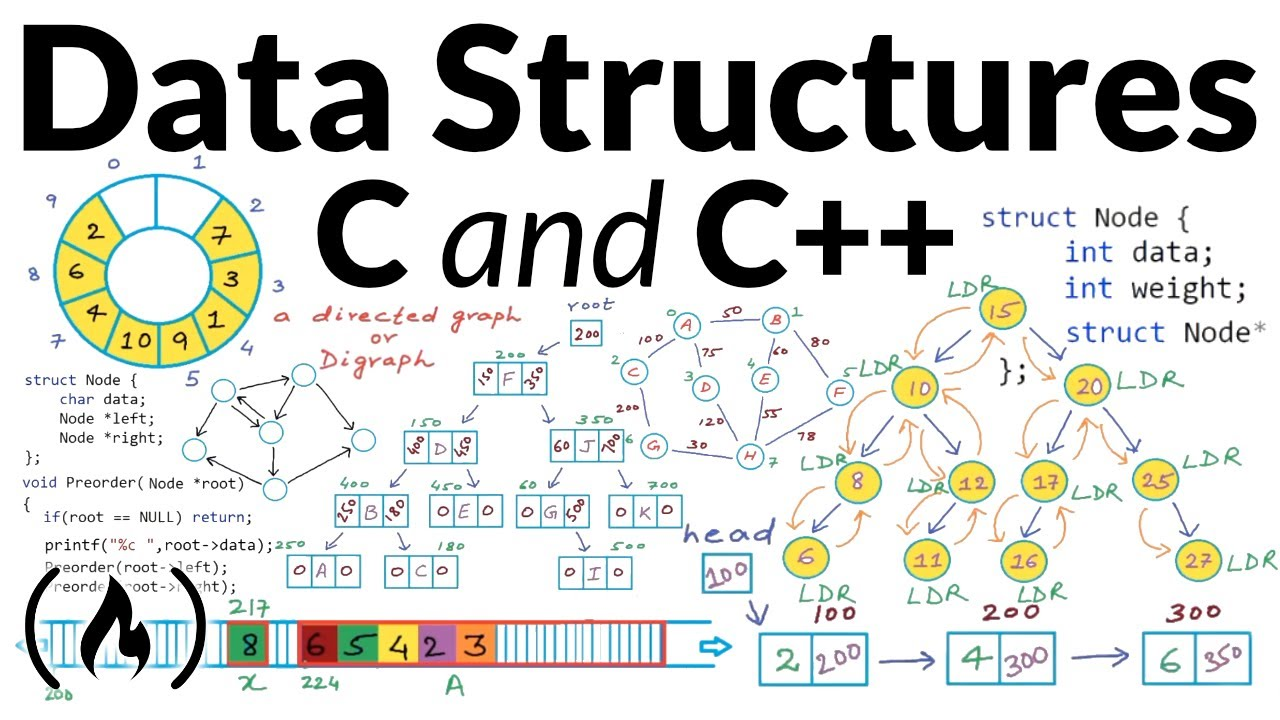
\includegraphics[width=0.8\textwidth]{assets/dataStructures.jpg}
    \caption{图片标题} % 图例,按章节编号
    \label{fig: 数据结构2} % 图片索引
\end{figure}

\subsection{多图并排}

\begin{figure}[H]
    \centering
    \begin{minipage}[c]{0.40\textwidth} %minipage使之保持同一行
    \centering
    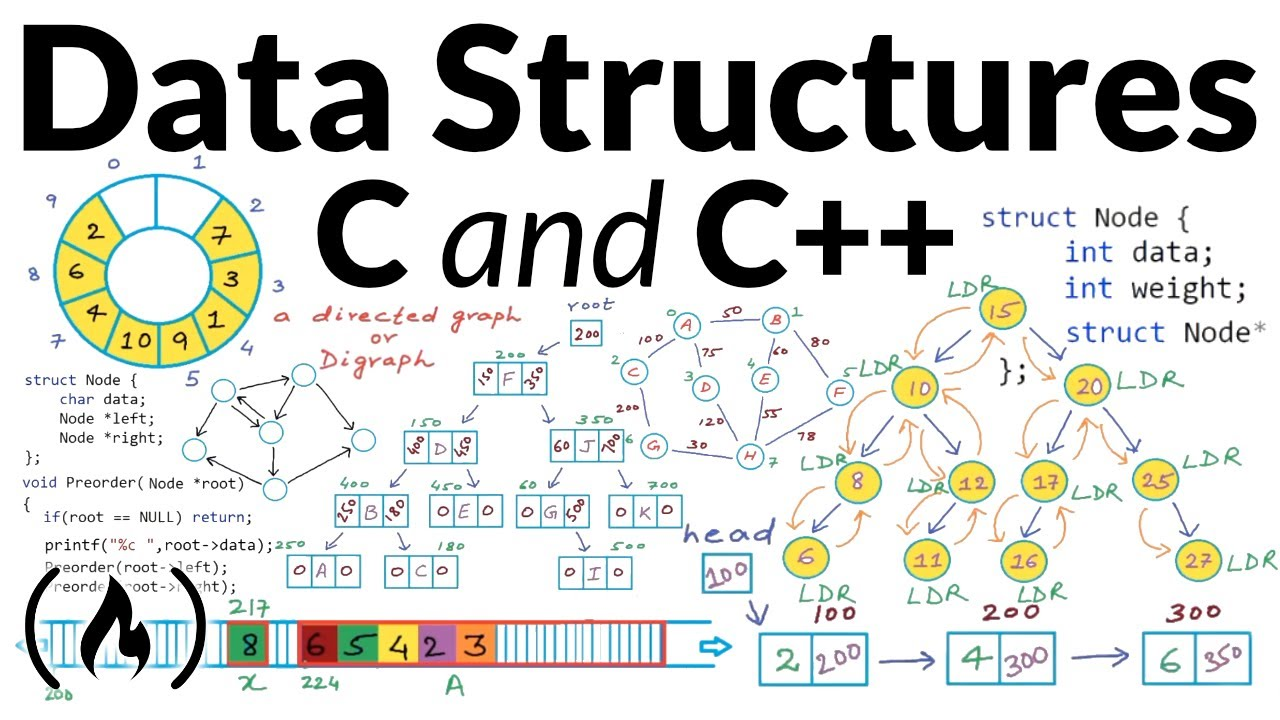
\includegraphics[width=0.8\textwidth]{assets/dataStructures.jpg}\\
    \caption{图片1标题}
    \end{minipage}
    \hspace{1em}
    \begin{minipage}[c]{0.40\textwidth} %minipage使之保持同一行
    \centering
    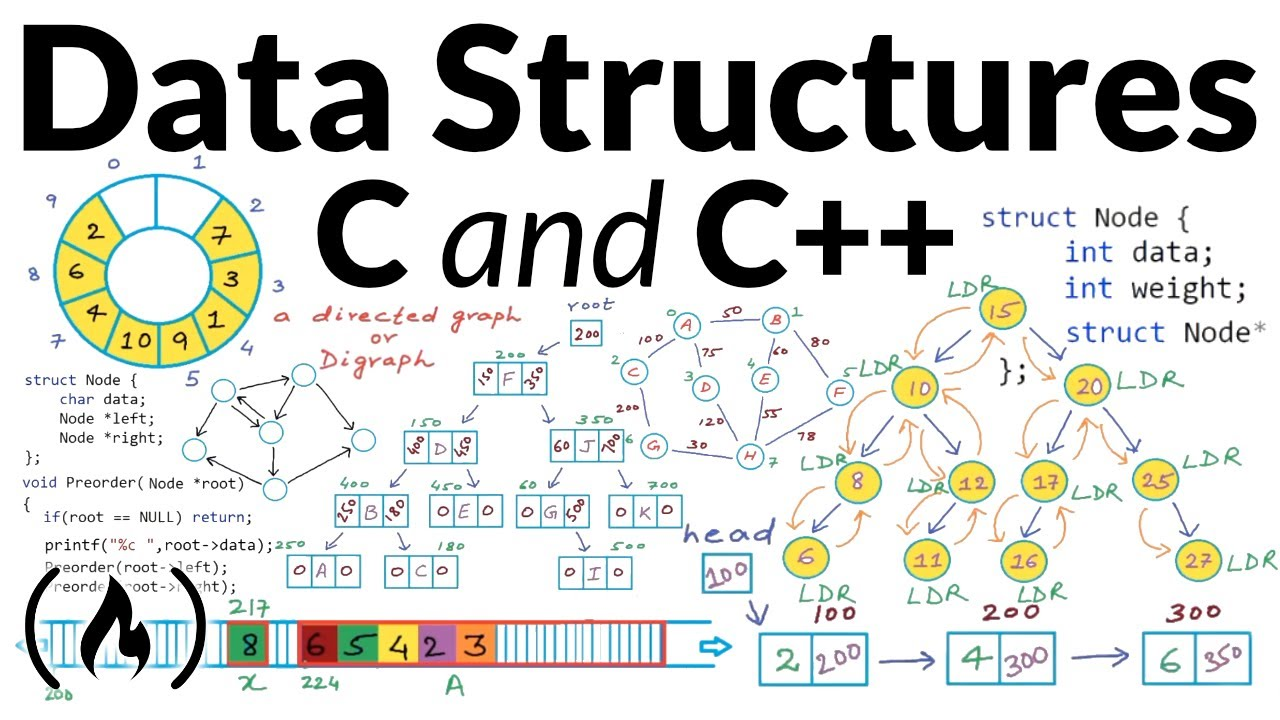
\includegraphics[width=0.8\textwidth]{assets/dataStructures.jpg}\\
    \caption{图片2标题}
    \end{minipage}
\end{figure}

\reSection{插入表格}
\subsection{一个表}

\begin{table}[H]
    \centering
    \caption{表格标题}
        \begin{tabular}{c||l}
        \toprule
        parameter  & Description \\
        \midrule
        $I$ & Land area collection \\
        $J$ & Flower pollination demand set \\
        $D_j$ & Number of pollinating bees required for flower pollination \\
        $T_k$ & Honeycomb size grade, $k = 1, 2, \cdots$ \\
        $B$ & Maximum number of hive \\
        $R_{ik}$ & Maximum influence radius of a single honeycomb \\
        \bottomrule
        \end{tabular}%
    \label{tab: 一个表}%
\end{table}%

\subsection{多表并排}

\begin{minipage}[c]{0.45\textwidth}
    \centering
    \begin{table}[H]
        \centering
        \caption{表格1标题}
            \begin{tabular}{c||lc}
            \toprule
            Symbol  & Description & Unit \\
            \midrule
            $t$ & $t_{th}$ year & $\sim$ \\
            $e_k$ & the error term & $\sim$ \\
            $X_{ij}$ & Raw data matrix & $\sim$ \\
            $Y_{ij}$ & Positive matrix & $\sim$ \\
            \bottomrule
            \end{tabular}%
        \label{tab: 表格1标题}%
    \end{table}%
\end{minipage}
\begin{minipage}[c]{0.45\textwidth}
    \centering
    \begin{table}[H]
        \centering
        \caption{表格2标题}
            \begin{tabular}{c||lc}
            \toprule
            Symbol  & Description & Unit \\
            \midrule
            $t$ & $t_{th}$ year & $\sim$ \\
            $e_k$ & the error term & $\sim$ \\
            $X_{ij}$ & Raw data matrix & $\sim$ \\
            $Y_{ij}$ & Positive matrix & $\sim$ \\
            \bottomrule
            \end{tabular}%
        \label{tab: 表格2标题}%
    \end{table}%
\end{minipage}

%%%%%%%%%%%%%%% 代码块 %%%%%%%%%%%%%%%
\reSection{插入代码}
\subsection{直接输入代码}

直接在 .tex 中输入代码,但不建议这种方式:

\begin{lstlisting}[language=c++,title={code.cpp}]
#include "bits/stdc++.h"

using namespace std;

int main() {
    cout << "3000ye 的 LaTeX 模板!" << endl;

    return 0;
}
\end{lstlisting}

\subsection{导入文件代码}

推荐使用文件导入代码,方便自动更新。

\lstinputlisting[language=c++, title=code.cpp]{code/code.cpp}

\reSection{伪代码}

\begin{algorithm}
    \caption{Example Pseudocode}
    \begin{algorithmic}
        \STATE $x\gets0$
        \IF {$x\leq 0$}
        \STATE $x\gets x+1$
        \ELSE
        \STATE $x\gets x-1$
        \ENDIF
    \end{algorithmic}
\end{algorithm}



%%%%%%%%%%%%%%% 参考文献 %%%%%%%%%%%%%%%
\section*{} % 参考文献
\reference{
    \bibitem{RN1} 参考文献
    \bibitem{RN2} 参考文献
}

%%%%%%%%%%%%%%% 致谢 %%%%%%%%%%%%%%%
\reThanks{
    致谢,3000ye 的 \LaTeX 模板!
}

\end{document}